\section{Конструкторский раздел}

В данном разделе приведены ключевые алгоритмы использовавшиеся при написании драйвера и демона с описанием в виде схем.

\subsection{Алгоритм обработки URB}

На рисунке \ref{alg:urb-dispatch} приведена схема алгоритма обработки URB.

\begin{figure}[ht]
    \centering
    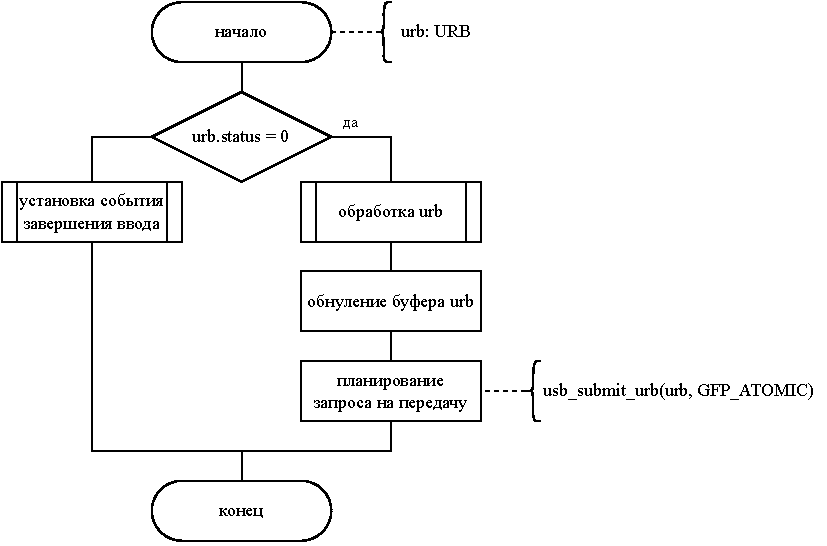
\includegraphics[keepaspectratio,width=\linewidth,height=0.85\textheight]{img/urb-dispatch.pdf}
    \caption{Схема алгоритма обработки URB}
    \label{alg:urb-dispatch}
\end{figure}

На рисунке \ref{alg:urb-handle} приведена схема алгоритма обработки корректного URB пакета и генерации необходимых сообщений о вводе.

\begin{figure}[ht]
    \centering
    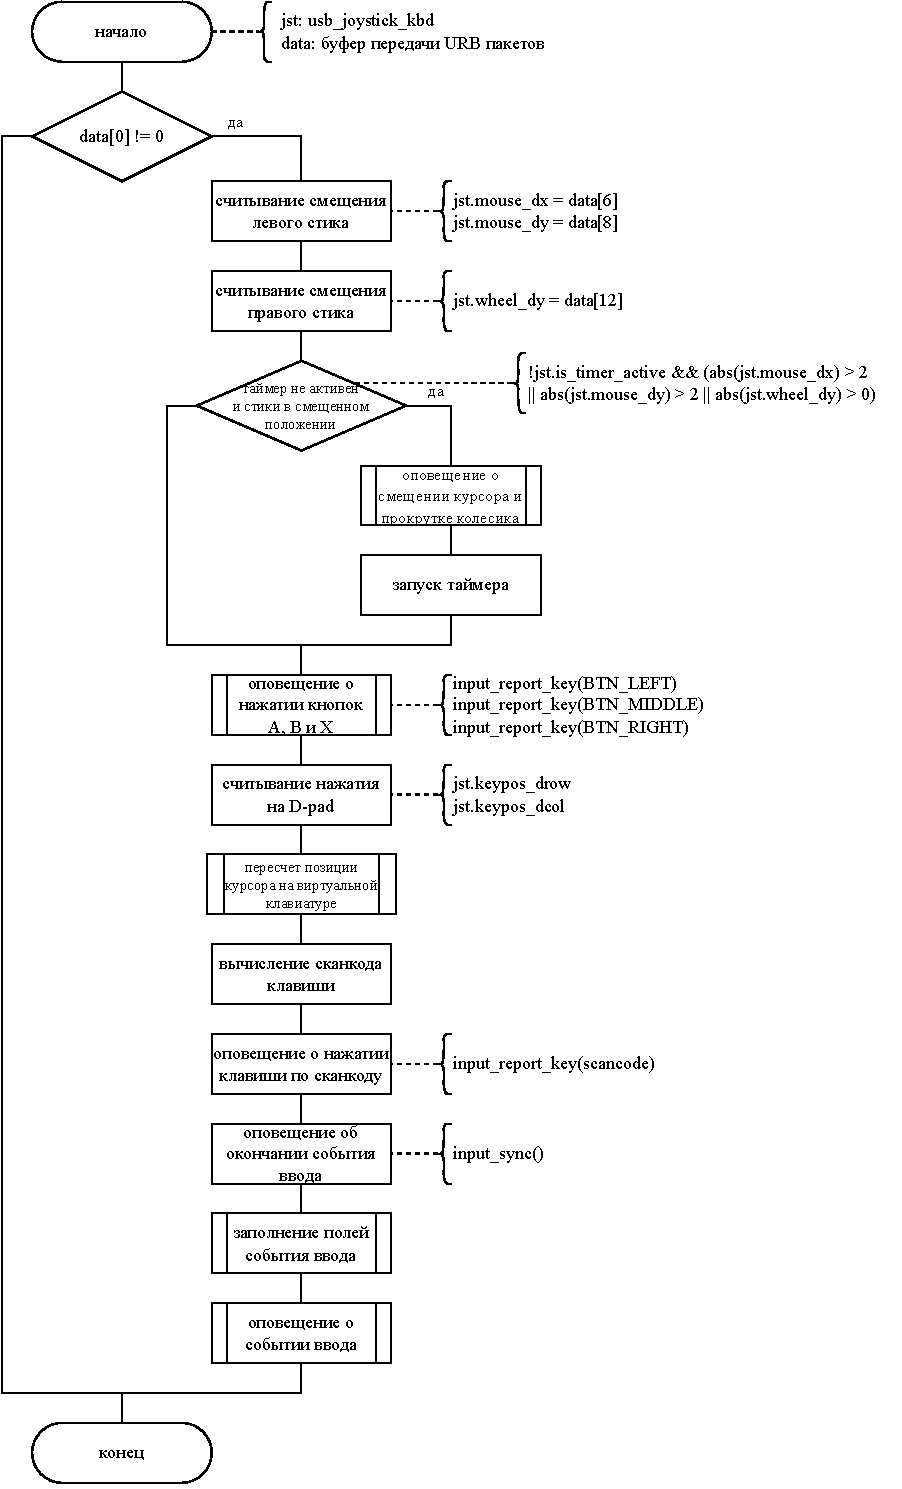
\includegraphics[keepaspectratio,width=\linewidth,height=0.85\textheight]{img/urb-handle.pdf}
    \caption{Схема алгоритма обработки корректного URB пакета}
    \label{alg:urb-handle}
\end{figure}

\clearpage

\subsection{Алгоритмы работы с событиями ввода}

На рисунке \ref{alg:emit-event} представлена схема алгоритма издания события с пробуждением ждущих процессов.

\begin{figure}[ht]
    \centering
    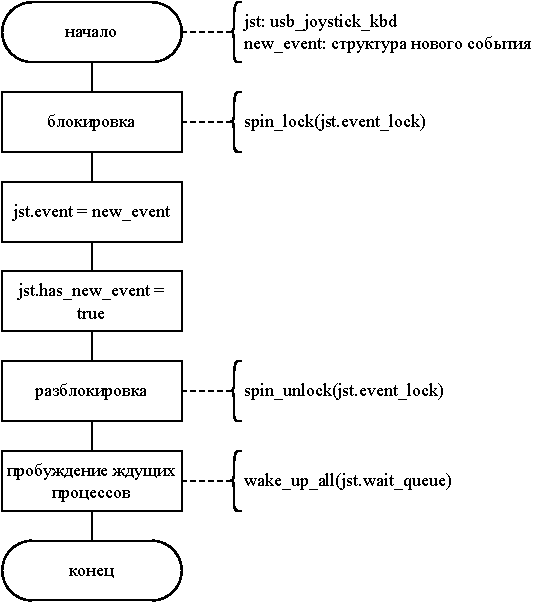
\includegraphics[keepaspectratio,width=0.75\linewidth,height=0.85\textheight]{img/emit-event.pdf}
    \caption{Схема алгоритма издания события}
    \label{alg:emit-event}
\end{figure}

На рисунке \ref{alg:proc-read} приведена схема алгоритма чтения события с блокировкой и ожиданием.

\begin{figure}[ht]
    \centering
    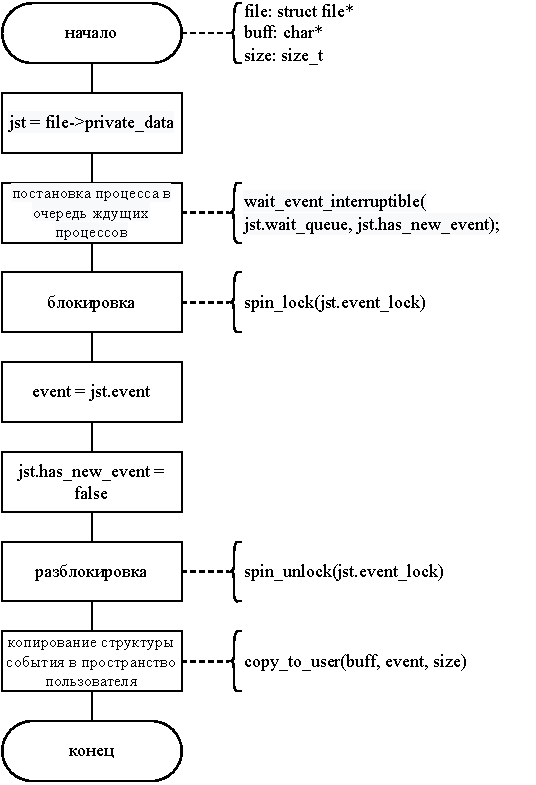
\includegraphics[keepaspectratio,width=\linewidth,height=0.85\textheight]{img/proc-read.pdf}
    \caption{Схема алгоритма чтения события из файла}
    \label{alg:proc-read}
\end{figure}

% TODO: алгоритм воркера в демоне

\pagebreak
